% ============================================================
%  tikz_fig_bc_cycle.tex  ── 下段パネルのみ（スライド2枚目用）
%  【使用例】
%    \begin{frame}{景気循環}
%      \input{tikz/tikz_fig_bc_cycle}
%    \end{frame}
% ============================================================
\documentclass[tikz, dvipdfmx]{standalone}
\usepackage{tikz}
\usepackage{pgfplots}
\pgfplotsset{compat=1.18}
\usepgfplotslibrary{fillbetween}
\usetikzlibrary{arrows.meta}
\definecolor{gdpblue} {RGB}{30,  90,  180}
\definecolor{trendred}{RGB}{190, 40,  40}
\definecolor{expgreen}{RGB}{200, 230, 200}
\definecolor{recred}  {RGB}{240, 200, 200}

\begin{document}
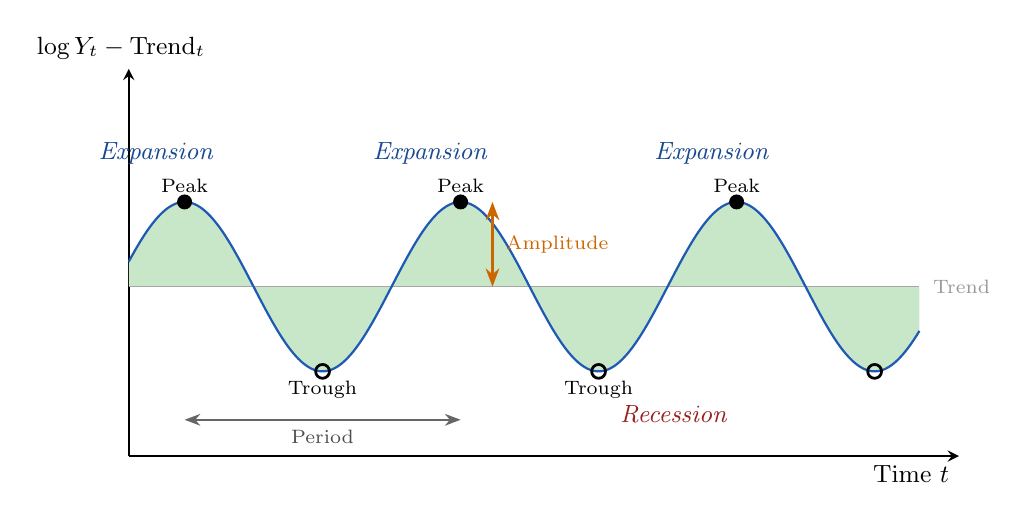
\begin{tikzpicture}
\begin{axis}[
  width  = \linewidth,
  height = 6.5cm,
  xmin = 0, xmax = 10.5,
  ymin = -1.4, ymax = 1.8,
  xtick = \empty, ytick = \empty,
  axis lines      = left,
  axis line style = {thick},
  clip            = false,
  every axis plot/.append style = {smooth},
  font = \small,
  %ylabel = {Cyclical component ($\log Y_t - \mathrm{Trend}_t$)},
  ylabel = {$\log Y_t - \mathrm{Trend}_t$},
  ylabel style = {
    rotate = -90,
    at     = {(axis description cs: -0.01, 1.0)},
    anchor = south east,
    xshift = 1.2cm,
  },
  xlabel = {Time $t$},
  xlabel style = {
    at     = {(axis description cs: 1.0, 0)},
    anchor = north east,
  },
]
  % ── fill between 用透明パス ─────────────────────────────
  \addplot[draw=none, name path=cycle_path, domain=0:10, samples=300]
    { 0.7*sin(deg(1.8*x + 0.3)) };
  \addplot[draw=none, name path=zero_path, domain=0:10] { 0 };

  % ── 拡張（緑）/ 後退（赤）シェーディング ────────────────
  \addplot fill between[
    of = cycle_path and zero_path,
    every even segment/.style = {fill=expgreen},
    every odd  segment/.style = {fill=recred},
  ];

  % ── ゼロ基準線 ──────────────────────────────────────────
  \addplot[gray!70, thin, domain=0:10] { 0 };
  \node[right, font=\scriptsize, gray!80]
    at (axis cs: 10.05, 0) {Trend};

  % ── 循環成分の線 ─────────────────────────────────────────
  \addplot[gdpblue, thick, domain=0:10, samples=300]
    { 0.7*sin(deg(1.8*x + 0.3)) };

  % ── 振れ幅の注釈 ─────────────────────────────────────────
  % Peak(x=4.197)での両矢印
  \draw[<->, thick, orange!80!black, >=Stealth]
    (axis cs: 4.6, 0) -- (axis cs: 4.6, 0.7);
  \node[right, font=\scriptsize, orange!80!black]
    at (axis cs: 4.65, 0.35) {Amplitude};

  % ── Peak ● ──────────────────────────────────────────────
  \addplot[only marks, mark=*, mark size=2.5pt,
    mark options={fill=black}]
    coordinates { (0.706,0.7) (4.197,0.7) (7.688,0.7) };
  \node[above, font=\scriptsize] at (axis cs: 0.706,  0.7) {Peak};
  \node[above, font=\scriptsize] at (axis cs: 4.197,  0.7) {Peak};
  \node[above, font=\scriptsize] at (axis cs: 7.688,  0.7) {Peak};

  % ── Trough ○ ─────────────────────────────────────────────
  \addplot[only marks, mark=o, mark size=2.5pt,
    mark options={fill=white, draw=black, line width=1pt}]
    coordinates { (2.451,-0.7) (5.942,-0.7) (9.433,-0.7) };
  \node[below, font=\scriptsize] at (axis cs: 2.451, -0.7) {Trough};
  \node[below, font=\scriptsize] at (axis cs: 5.942, -0.7) {Trough};

  % ── 周期を示す両矢印 ─────────────────────────────────────
  % Peak(0.706) → Peak(4.197) の間
  \draw[<->, semithick, black!60, >=Stealth]
    (axis cs: 0.706, -1.1) -- (axis cs: 4.197, -1.1);
  \node[below, font=\scriptsize, black!70]
    at (axis cs: 2.45, -1.1) {Period};

  % ── Expansion / Recession ラベル ─────────────────────────
  \node[font=\small, gdpblue!80!black]
    at (axis cs: 0.353,  1.1) {\textit{Expansion}};
  \node[font=\small, trendred!80!black]
    at (axis cs: 2.45,  -1.1) {};  % Periodラベルと重なるので省略
  \node[font=\small, gdpblue!80!black]
    at (axis cs: 3.82,   1.1) {\textit{Expansion}};
  \node[font=\small, trendred!80!black]
    at (axis cs: 5.942, -1.1) {};
  \node[font=\small, gdpblue!80!black]
    at (axis cs: 7.38,   1.1) {\textit{Expansion}};

  % Recession ラベル（Periodラベルと重ならない位置に）
  \node[font=\small, trendred!80!black]
    at (axis cs: 6.9, -1.05) {\textit{Recession}};

\end{axis}
\end{tikzpicture}
\end{document}
